\documentclass[a4paper,11pt,leqno]{article} \usepackage{amsmath}
\usepackage{amsfonts} \usepackage{amsthm} \usepackage{amssymb}
%\usepackage{slashbox} \usepackage{tikz-cd}
\usepackage{mathrsfs} \DeclareMathAlphabet{\mathpzc}{OT1}{pzc}{m}{it}
\usepackage{graphicx} \usepackage{hyperref}
%\DeclareGraphicsExtensions{.png,.jpeg} \usepackage[bottom=1.5in, left=1.25in,
%right=1.25in, top=1.5in]{geometry}
\usepackage[bottom=1in, left=1in, right=1in, top=0.9in]{geometry}
%\usepackage{fancyhdr}
\usepackage{mathtools} \usepackage{color} \usepackage{enumitem}
\usepackage{amsthm} \usepackage{tikz}
\usetikzlibrary{decorations.markings,arrows}
%\usepackage{pgfplots} \usepackage{fancyvrb} \usepackage{linalgjh}
\usepackage{subcaption}

\DeclarePairedDelimiter{\floor}{\lfloor}{\rfloor}
%\pagestyle{fancy}
\renewcommand{\d}{\ensuremath{\operatorname{d}}}
\newcommand*{\Comb}[2]{{}^{#1}C_{#2}}% \newcommand{\sub}{\subseteq}
\newcommand{\lto}{\leftarrow} \newcommand{\inj}{\xhookrightarrow{}}
\newcommand{\NN}{\mathbb{N}} \newcommand{\ZZ}{\mathbb{Z}}
\newcommand{\CC}{\mathbb{C}} \newcommand{\ZP}{\mathbb{Z}_p}
\newcommand{\RR}{\mathbb{R}} \newcommand{\QQ}{\mathbb{Q}}
\newcommand{\FF}{\mathbb{F}} \newcommand{\curA}{\mathscr{A}}
\newcommand{\curB}{\mathscr{B}} \newcommand{\curC}{\mathscr{C}}
\newcommand{\curD}{\mathscr{D}} \newcommand{\curI}{\mathscr{I}}
\newcommand{\curM}{\mathscr{M}} \newcommand{\of}{\circ}
\newcommand{\sub}{\subseteq} \newcommand{\XOR}{\otimes}
\newcommand{\car}[1]{\overline{\overline{#1}}}
\renewcommand{\Re}{\ensuremath{\operatorname{Re}}}
\renewcommand{\Im}{\ensuremath{\operatorname{Im}}}
\newcommand{\id}{\ensuremath{\operatorname{id}}}
\newcommand{\im}{\ensuremath{\operatorname{im}}}
\newcommand{\Hom}{\ensuremath{\operatorname{Hom}}}
\newcommand{\Ext}{\ensuremath{\operatorname{Ext}}}
\newcommand{\ev}{\ensuremath{\operatorname{ev}}}
\newcommand{\Obj}{\ensuremath{\operatorname{Obj}}}
\newtheorem*{thm}{Theorem}
\newtheorem*{lemma}{Lemma}
\newtheorem{prop}{Proposition}
\theoremstyle{definition}
\newtheorem{defn}{Definition}
\newcommand{\divides}{\bigm|} \newcommand{\notdivides}{% \mathrel{\mkern.5mu
  % small adjustment
  % superimpose \nmid to \big|
    \ooalign{\hidewidth$\big|$\hidewidth\cr$\nmid$\cr}% }%
    } \newcommand{\norm}[1]{\left\lVert#1\right\rVert}
    \newcommand{\Res}{\text{Res}} \newcommand{\del}{\partial}

\title{The mathematics of UMAP} \author{Adele Jackson}
\begin{document}
\thispagestyle{empty}
\maketitle

\section{Introduction}

UMAP (Uniform Manifold Approximation and Projection) is a new dimension
reduction technique~\cite{McInnes18}, currently
implemented~\cite{McInnesGithub, MelvilleGithub} for both labelled and
unlabelled data.
Figure~\ref{fig_example_embedding} shows a comparison of UMAP embeddings with
the outputs of some other standard dimension reduction algorithms.
UMAP gives similarly good outputs for visualisation as t-SNE, with
a substantially better runtime (see~\cite{McInnesBenchmarking}), and may
capture more of the global structure of the data.
The current UMAP implementation also allows UMAP to be used as a preprocessing
step in a machine learning pipeline, as new data can be embedded into an
existing model.

\begin{figure}
  \centering
  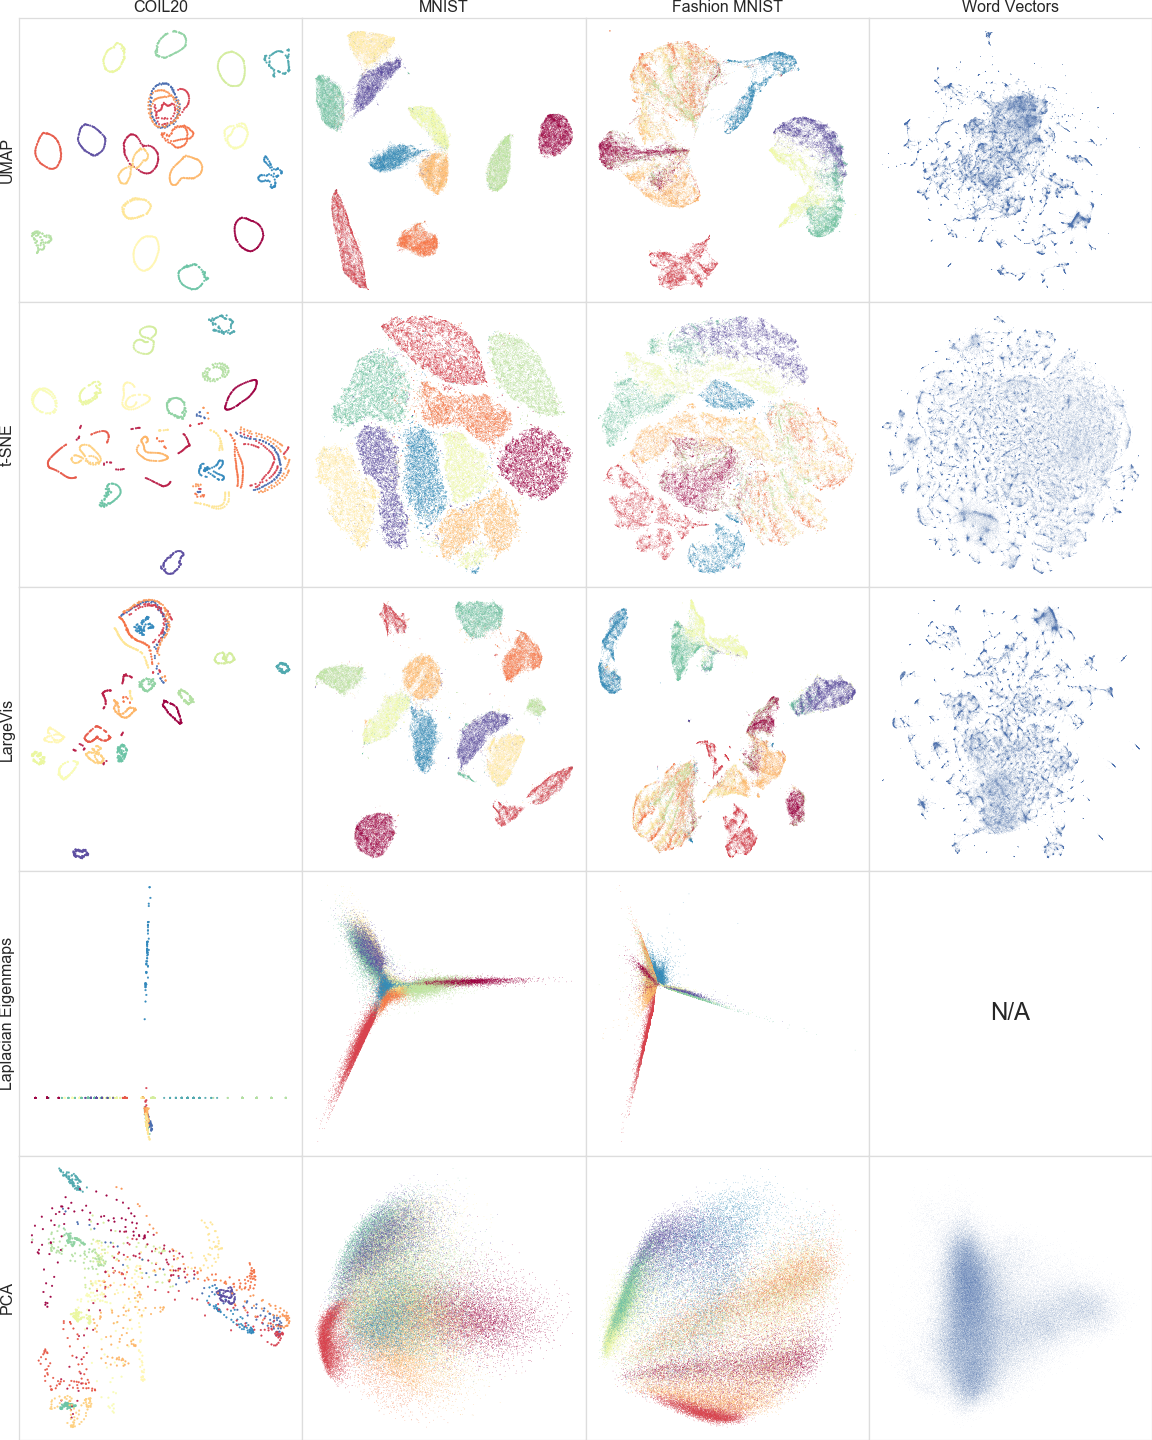
\includegraphics[width=1.05\textwidth]{figures/dim-red-comparison-nips.png}
  \caption{Embeddings from UMAP, t-SNE, LargeVis, Laplacian Eigenmaps and PCA
  on some standard datasets. Image taken from~\cite{McInnes18}.}
  \label{fig_example_embedding}
\end{figure}

Excitingly, UMAP is based on strong and general mathematical theory, which does
not depend on a Euclidean metric.
As a result, UMAP can be used for datasets with a mixture of categorical and
continuous features.

The main mathematical result behind UMAP is that there is an adjunction between
finite fuzzy simplicial sets and finite extended pseudo-metric spaces.
In this document, we will explain what this statement means and why it is
useful.

Given a dataset $D$ in $\RR^N$, we wish to find a good representation of $D$ in
a lower-dimensional space, $\RR^m$.
We wish to develop a good loss function for evaluating a lower-dimensional
representation, so we can minimise this loss.
To do this, we will construct a fuzzy simplicial set from a dataset.
A fuzzy simplicial set (which we will define in Section~\ref{section_fss}) is
an abstract description of a topological space, with probabilities on its
elements that we will interpret as giving their size.
We will build a partially-defined metric space relative to each vertex, then
use the adjunction to convert this family of metric spaces to a family of fuzzy
simplicial sets.
In the algorithm, this step corresponds to constructing the adjacency matrix
$A$ for a weighted directed graph~\cite[Section 3.1]{McInnes18}.
We then take a union of this family, which corresponds to constructing the
symmetric matrix $B = A+A^T-A\circ A^T$ where $\circ$ is the Hadamard product.
We can then compare the fuzzy simplicial set from our dataset $D$ with that
from a proposed low-dimensional representation, to find the low-dimensional
representation that minimises the cross entropy loss between the two fuzzy
sets.

\section{Approximating the underlying manifold}
\label{section_uniform}

Given a dataset $D$ in $\RR^N$, we think of the datapoints as being drawn from
some Riemannian manifold\footnote{
  A Riemannian manifold is a space that locally looks like Euclidean space, in
  which we have well-defined notions of distances, angles, and volumes.
  For example, the surface of a unit sphere in $\RR^3$ is a two-dimensional
  Riemannian manifold.
} $M$, then mapped into $\RR^N$ by some injective map $\phi: M\to\RR^N$.
See Figure~\ref{fig_M_in_Rn} for an illustration of this setup.

One approach to finding a low-dimensional representation of $D$ is to
reconstruct $M$, then find a good map from $M$ into $\RR^m$.
To do this, we assume that $D$ is uniformly drawn from $M$, as in
the example in Figure~\ref{fig_M_in_Rn}.
(Note that parts of $M$ might be stretched out or compressed under the map
$\phi$ into $\RR^N$, so this does {\textbf{not}} imply that the data is
uniformly distributed in $\RR^N$.)
This assumption means that $D$ approximates $M$ well.
(This is also where the `U' in UMAP comes from.)

\begin{figure}
    \centering
    \begin{subfigure}[b]{0.45\textwidth}
        $$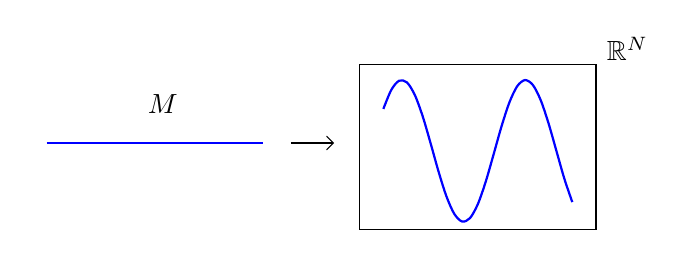
\begin{tikzpicture}
            \node (A) at (-1.1,2) {};
            \node (B) at (1.9,2) {};
            \node (C) at (0.5,2.5) {$M$};
            \node (D) at (2,2) {};
            \node (E) at (2.8,2) {};
            \node (F) at (6.4, 3.2) {$\RR^N$};
            {\path[-, thick, color=blue] (A) edge node[above]{} (B);}
            \path[->,font=\small,>=angle 90] (D) edge node[left]{} (E);
            \draw (3, 0.9) rectangle (6, 3);
            \draw plot[domain=3.3:5.7,smooth] (\x,{0.9*sin(4*\x r)+1.9})[thick, color=blue];
        \end{tikzpicture}$$
        \caption{The manifold $M$ embedded in $\RR^N$.}
    \end{subfigure}
    \begin{subfigure}[b]{0.45\textwidth}
        $$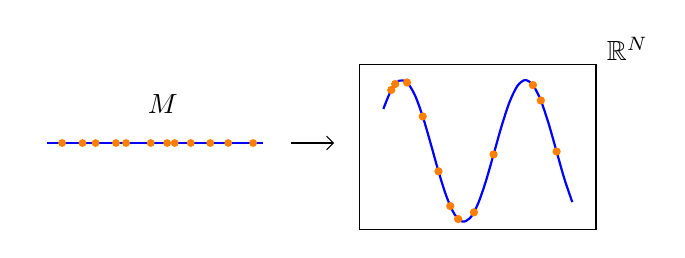
\begin{tikzpicture}
            \pgfmathsetseed{20}
            \node (A) at (-1.1,2) {};
            \node (B) at (1.9,2) {};
            \node (C) at (0.5,2.5) {$M$};
            \node (D) at (2,2) {};
            \node (E) at (2.8,2) {};
            \node (F) at (6.4, 3.2) {$\RR^N$};
            {\path[-, thick, color=blue] (A) edge node[above]{} (B);}
            \path[->,font=\small,>=angle 90] (D) edge node[left]{} (E);
            \draw (3, 0.9) rectangle (6, 3);
            \draw plot[domain=3.3:5.7,smooth] (\x,{0.9*sin(4*\x r)+1.9})[thick, color=blue];
            \foreach \i in {3.4,3.45,3.6, 3.8, 4.0, 4.15, 4.25, 4.45, 4.7, 5.2, 5.3, 5.5} {
                \fill[orange] (\i,{0.9*sin(4*\i r)+1.9}) circle (1.5pt);
            }
            \foreach \i in {1,...,12} {
                \node at (0.21428*\i-1+0.075*rand, 2)[circle,fill=orange, inner sep=1pt] {};
            }
        \end{tikzpicture}$$
        \caption{The dataset $D$ is uniformly drawn from $M$.}
    \end{subfigure}
    \begin{subfigure}[b]{0.45\textwidth}
        $$\begin{tikzpicture}
            \pgfmathsetseed{20}
            \node (A) at (-1.1,2) {};
            \node (B) at (1.9,2) {};
            \node (C) at (0.5,2.5) {$D$};
            \node (D) at (2,2) {};
            \node (E) at (2.8,2) {};
            \node (F) at (6.4, 3.2) {$\RR^N$};
            \path[->,font=\small,>=angle 90] (D) edge node[left]{} (E);
            \draw (3, 0.9) rectangle (6, 3);
            \foreach \i in {3.4,3.45,3.6, 3.8, 4.0, 4.15, 4.25, 4.45, 4.7, 5.2, 5.3, 5.5} {
                \fill[orange] (\i,{0.9*sin(4*\i r)+1.9}) circle (1.5pt);
            }
            \foreach \i in {1,...,12} {
                \node at (0.21428*\i-1+0.075*rand, 2)[circle,fill=orange, inner sep=1pt] {};
            }
        \end{tikzpicture}$$
        \caption{We see only $D$.}
    \end{subfigure}
    \caption{The dataset is drawn from a manifold embedded in $\RR^N$.}
    \label{fig_M_in_Rn}
\end{figure}

Note that we have two notions of distance between our datapoints: the distance
from $\RR^N$, and the ``true'' distance in $M$.
To reconstruct $M$, we wish to reconstruct this second distance.
We now formally define the mathematical object we wish to reconstruct.

\begin{defn}
  A \emph{metric} on a set of points $X$ is a function $d: X\times X\to \RR$
  that satisfies the following conditions.
  First, the metric is non-negative: $d(x, y) \geq 0$ for all $x, y\in X$.
  Second, the function is symmetric: $d(x, y) = d(y, x)$ for all $x, y\in X$.
  Third, the function distinguishes points: $d(x, y) = 0$ if and only if $x
  = y$.
  Finally, a metric satisfies the triangle inequality: $d(x, z)\leq d(x, y)
  + d(y, z)$ for all $x,y,z\in X$.
\end{defn}

The words ``metric`` and ``distance function`` are interchangeable.
A \emph{metric space} is a the pair $(X, d)$, where $X$ is a set of points and
$d$ is a metric for $X$.

If we assume that the metric on $M$ is locally constant, we get the following
lemma.
We will show that this lemma allows us to approximate the distance between two
points $x, y\in D$ as measured in $M$, so long as $x$ and $y$ are close enough
in $\RR^N$, by normalising by the distance from $x$ to its $k$-nearest
neighbour.

\begin{lemma}[\cite{McInnes18}]
  Let $(M, g)$ be a Riemannian manifold\footnote{
    In this, $M$ is the manifold and $g$ is a two-form that gives us measures of
    distance, volumes and angles.
  } embedded in $\RR^n$.
  Let $p\in M$ be a point.
  Suppose that $g$ is locally constant.\footnote{
    To be precise, we assume that there is an open neighbourhood $U$ with
    $p\in U$ on which $g$ is locally constant, such that $g$ is a constant
    diagonal matrix in the ambient coordinates.
  }
  Let $B$ be a ball in $M$, containing $p$, whose volume is
  $\frac{\pi^{n/2}}{\Gamma(n/2+1)}$ with respect to the metric on $M$.
  Then the distance of the shortest path in $M$ from $p$ to a point $q\in B$ is
  $\frac{1}{r}d_{\RR^n}(p, q)$, where $r$ is the radius of $B$ in $\RR^n$ and
  $d_{\RR^n}(p, q)$ is the distance from $p$ to $q$ in $\RR^n$.
\end{lemma}

We approximate distances in $M$ between nearby datapoints as follows.
Fix a radius $R$.
As the dataset $D$ is uniformly distributed in $M$, the expected number of
datapoints in any radius $R$ ball in $M$ is some constant $k$.
Now, for $x\in D$, let $N_k(x)$ be the ball in $\RR^N$, centred at $x$, that
contains its $k$ nearest neighbours.
Let $\tilde{N}_k(x)$ be the preimage of $N_k(x)$ in $M$ (this is $\phi^{-1}(N_k(x))$).
If $k$ is small enough that $g$ is locally constant on $\tilde{N}_k(x)$, then
this preimage will be a ball of some radius, and the expected value of this
radius will be $R$.
By the lemma we can reconstruct
distances within $N_k(x)$ by normalising by $\frac{R}{r_x}$ where $r_x$ is the
distance from $x$ to its $k$-nearest neighbour
As we only care about distances up to a constant factor, it suffices to
normalise by $r_x$ in each of the $N_k(x)$ for $x\in D$.

Thus, by the lemma, we can approximate distances from $x$ to points in $N_k(x)$
as follows.
Fix a value of $k$.
Now we can calculate the distance in $M$, based at $x_i$, from $x_i$ to $x_j$
to be approximately
$$\frac{1}{r_i}d_{\RR^N}(x_i, x_j),$$
where $r_i$ is the distance from $x_i$ to its $k^{th}$-nearest neighbour.
To reduce the impact of noise in the distribution of datapoints on the value of
$r_i$, in practice we take $r_i$ to be the value such that
$$\sum_{j=1}^k\exp\left(\frac{-|x_i-x_{i_j}|}{r_i}\right) = \log_2(k)$$
where $\{x_{i_1},\ldots,x_{i_k}\}$ are the $k$ nearest neighbours of $x_i$.

We now modify these distances in two ways.
Note that the distance in $M$, based at $x_i$, from $x_j$ to $x_k$ for
$j,k\not= i$ is not defined.
We set this to $\infty$ to signal this.
To avoid having isolated points, we also assume the manifold is locally
connected, so has no isolated points, and that there are enough datapoints that
no datapoint is in its own connected component.
To enforce this, let $\rho_i$ be the distance from $x_i$ to its nearest
neighbour.
Then we set
$$d_{x_i}(x_i, x_j)=\frac{1}{r_i}\max(0, d_{\RR^N}(x_i,
x_j)-\rho_i).$$
The effect of this modification is to force the distance from $x_i$ to its
nearest neighbour to be 0.

Following this process gives us an \emph{extended pseudo-metric space} for each
choice of $x_i$.
We get an extended pseudo-metric, rather than a metric, as some of our
distances are infinite and some distances between distinct points are zero.
\begin{defn}
  An \emph{extended pseudo-metric space} is a set $X$ with a function $d:
  X\times X\to \RR \cup \{\infty\}$ satisfying the following conditions.
  First, the metric is non-negative and symmetric.
  Second, $d(x, x) = 0$ for all $x$.
  Finally, let $x,y,z\in X$.
  Then either $d(x,z) = 0$, or $d(x,z)\leq d(x,y)+d(y,z)$.
\end{defn}
The word ``pseudo`` refers to the weakening of the condition that $d(x,y) = 0$
if and only if $x = y$, and ``extended`` refers to the addition of the value
$\infty$.

This setup presents us with a problem.
The distance we get from $x_i$ to $x_j$ using this method will in general be
different to that from $x_j$ to $x_i$, as $r_j\not= r_i$.
This is due to the fact that, while the $x_i$ are uniformly drawn from the
manifold, they are not all the same distance apart.
We need a technique for combining a family of locally-defined finite metric
spaces to get a global structure.
This is where we will use the adjunction between extended pseudo-metric spaces
and fuzzy simplicial sets.

Note that, although we have used the $\RR^N$ metric to develop this theory, the
idea still holds with any other metric.
As a result, UMAP can be used with custom distance measures and can handle
categorical data and other measures of distance between datapoints.

\section{Category theory and adjunctions}

We will now define what an adjunction is, and set up the background for fuzzy
simplicial sets.

Category theory is a branch of mathematics that unifies common concepts across
different parts of mathematics.
For example, one can take the product of two vector spaces, or the product of
two sets, or two groups.
Using ideas from category theory, we can give one unified definition of a
``product'', with all these products as special cases, and prove results about
it that are valid independently of the specific context.

An adjunction is a translation between different domains of discourse.
For UMAP, the adjunction will let us move from a family of metric spaces to
a family of fuzzy simplicial sets, where we can take a union, in
a mathematically sound way.
Before we can define this translation, we will set up some fundamental category
theory concepts.\footnote{
  See~\cite{Spivak18} for a more detailed exposition of this material aimed at
  scientists.  We follow~\cite{Riehl} for these definitions.
}

\begin{defn}
  A \emph{category} $\curC$ is a collection of \emph{objects}, $\Obj(\curC)$,
  and between each $X, Y\in\Obj(\curC)$, a collection of \emph{morphisms}
  $\Hom_{\curC}(X, Y)$, that satisfy the following conditions.
  (We write $f: X\to Y$ to mean $f\in \Hom_{\curC}(X, Y)$.)

  First, we can \emph{compose} morphisms.
  Let $f: X\to Y$ and $g: Y\to Z$ be morphisms.
  Then there is a specified composite morphism $gf: X\to Z$.
  Furthermore, composition is \emph{associative}.
  Let $f: X\to Y$, $g: Y\to Z$ and $h: Z\to W$ be morphisms.
  Then $h(gf) = (hg)f$.

  Second, for each object $X$, there is a specified \emph{identity} morphism
  $1_X: X\to X$.
  Identity morphisms act as the identity under composition.
  That is, for any $f: X\to Y$, $1_Yf = f1_X = f$.
\end{defn}

One familiar example of a category is $\textbf{Vect}$.
This is the category whose objects are real vector spaces (of all dimensions),
where the morphisms between two vector spaces $V$ and $W$ are the linear
transformations $V\to W$.
Another example is $\textbf{Set}$, whose objects are sets, and morphisms are
functions between sets.

We can define \emph{functors} that let us transform objects and morphisms between them in
one category to those in another category.

\begin{defn}
  Let $\curC$ and $\curD$ be categories.
  A \emph{functor} $F: \curC\to \curD$ is a map from the objects and morphisms
  of $\curC$ to those of $\curD$ that respects the structure of $\curC$ in the
  following ways.
  The functor $F$ must preserve composition, so for all composable morphisms
  $g$ and $f$, $F(gf) = F(g)F(f)$.
  It also must fix identities, so that $F(1_X) = 1_{F(X)}$.
\end{defn}

We give some examples of functors between $\textbf{Vect}$ and $\textbf{Set}$.
For any category $\curC$, we have the identity functor $\id_{\curC}:
\curC\to \curC$ that fixes all objects and morphisms.

There is a ``forgetful'' functor $Forget: \textbf{Vect}\to \textbf{Set}$ that
takes a vector space to underlying set of its vectors, and a linear map to the
set map on the underlying sets of the vector spaces.
For example, $Forget$ takes the vector space $\RR$ to the set $\{\lambda\,|\,
\lambda\in\RR\}$.
For an example of its action on morphisms, it takes the map $f: \RR\to\RR$
mapping $(1)$ to $(2)$ to the map
$Forget(f): \{\lambda\,|\,\lambda\in\RR\}\to \{\lambda\,|\,\lambda\in\RR\}$
that takes $\lambda$ to $2\lambda$.
Note that there are many more maps from $Forget(f)$ to $Forget(f)$ than the
ones that come from linear transformations.
For example, the map taking $2\mapsto 4$ and all other $\lambda\in Forget(f)$
to $0$ is a valid map of sets, but is not the image under $Forget$ of
a morphism in $\textbf{Vect}$.

Note that there is no way to reverse $Forget$, as once we have applied it to
a vector space, there is no way to reconstruct the sums or scalar multiples of
vectors, or to recover a basis.
We might hope to find a functor $F: \textbf{Vect}\to\textbf{Set}$ that we can
reverse.
For example, we might wish to construct a functor $F$ that takes a vector space
$V$ to a particular basis for it.
However, even if there were some way to canonically choose a basis for each
vector space, this would not naturally give us a functor.
This is as there is no nice morphism between sets of basis elements to send,
for example, the linear transformation $v\mapsto 2\cdot v$ to.

A particularly nice functor going in the other direction is $Free:
\textbf{Set}\to \textbf{Vect}$.
This functor takes a set $\{x_i\}_{i\in I}$ to the free vector space on its
elements with real coefficients.
Now we can take any morphism $f: X\to Y$ between sets to a linear
transformation in a canonical way, by letting $Free(f): Free(X)\to Free(Y)$
take the basis element $Free(x_i)\in Free(X)$ to the basis element
$Free(f(x_i))\in Free(Y)$.
As a linear transformation is uniquely determined by its action on a basis for
the vector space, this is well-defined.

Two functors $F: \curC\to\curD$ and $G: \curD\to\curC$ form an
\emph{adjunction} if they translate between the two categories in a compatible
way.
The adjunction between finite fuzzy simplicial sets and finite extended
pseudo-metric spaces will allow us to take our family of finite extended
pseudo-metric spaces, each defined relative to a datapoint, and convert it to
a family of finite fuzzy simplicial sets, 
The functors $F$ and $G$ give us an adjunction if there is a particularly nice
pair of \emph{natural transformations} between $FG$ and the identity on
$\curD$, and between $GF$ and the identity on $\curC$.

A natural transformation lets us compare two functors $F, G:
\curC\to\curD$.
One motivating example for wanting to compare functors is the natural
isomorphism of a vector space with its double dual.
The double dual functor takes a vector space $V$ to its double dual $V^{**}$ by
mapping $v\in V$ to the map $f\mapsto f(v)$, which is evaluation at $v$.
The functor takes a linear transformation $T: V\to W$ to the double dual of the
linear transformation, which is defined by
$$T^{**}(\phi)(f)(v) = \phi\of (T^*(f))(v) = \phi\of f\of T(v).$$
The statement that the map taking $V$ to $V^{**}$ is a ``natural isomorphism'' can
be formalised by saying that there is a natural transformation from
the identity functor on $\textbf{Vect}$ to the double dual functor, that is an
isomoprhism on all the objects.
A natural transformation is defined as follows.

\begin{defn}
  Let $\curC$ and $\curD$ be categories, with $F, G: \curC\to \curD$ functors
  between them.
  A \emph{natural transformation} $\alpha: F\to G$ is a morphism
  $\alpha_X: FX\to GX$ for each $X\in \Obj(\curC)$ such that for any
  $f: X\to Y$ in $\curC$, $Gf\of \alpha_X = \alpha_Y\of Ff: FX\to GY$.
\end{defn}

Some intuition behind this is that a natural transformation $\alpha$ gives maps
between the images of the two functors that are compatible with all the
images of the morphisms between them, without knowing anything about these
morphisms. 

One useful thing that we can do with natural transformations is to make a new
category from any pair of categories $\curC$ and $\curD$.
We can compose natural transformations as follows.
Let $F, G, H$ be functors $\curC\to \curD$, with $\alpha$ a natural
transformation from $F$ to $G$, and $\beta$ one from $G$ to $H$.
Then there is a natural transformation $\beta\of\alpha$ from $F$ to $H$ with
$(\beta\of\alpha)_X = \beta_X\of\alpha_X$.
One can check that there is a category whose objects are functors
$\curC\to\curD$, and whose morphisms are natural transformations between them.

We can now define an adjunction.
Suppose we wish to translate between two categories $\curC$ and $\curD$, using
two functors $F: \curC\to \curD$ and $G: \curD\to\curC$.
We wish to define a condition on these functors for them to be a good pair of
translations.
We could ask that $F$ and $G$ give us an equivalence of categories; i.e. that
$GF = 1_{\curC}$ and $FG = 1_{\curD}$.
However, this is generally too strong a requirement, as the interesting case is
when we wish to translate between inequivalent categories (e.g. between sets
and vector spaces, or topological spaces and simplicial sets).
An adjunction is a weakening of this equivalence idea. 

\begin{defn}
  The functors $F: \curC\to\curD$ and $G: \curD\to\curC$ form an adjunction,
  notated by $F\dashv G$, if there are natural transformations $\eta:
  1_\curC\to GF$ and $\epsilon: FG\to 1_\curD$ satisfying the following 
  commutativity conditions:
  $$\epsilon_{F(c)}\of F(\eta_c) = \id_{F(c)}\text{ and} $$
  $$G(\epsilon_d)\of \eta_{G(d)} = \id_{G(d)}$$
  for all $c\in\curC$, $d\in\curD$.
\end{defn}

Note that this definition is not symmetric in $F$ and $G$ (hence why we use the
asymmetric notation $F\dashv G$).
One can show~\cite[Section 4]{Riehl} that an equivalent definition is that
$F\dashv G$ if there is an isomorphism between $Hom_\curD(F(c), d)$ and
$Hom_\curC(c, G(d))$ that is natural in both $c$ and $d$.

One example of an adjunction is between the free and forgetful functors between
$\textbf{Vect}$ and $\textbf{Set}$.
These categories are not equivalent.
However, we have $Free\dashv Forget$ where these functors are those defined
earlier in this section.
It is straightforward to check that there is a canonical bijection between the
morphism sets.

Finally, given a category $\curC$, we will define the opposite category $\curC^{op}$,
which we will use in the next section.
\begin{defn}
  Let $\curC$ be a category.
  The \emph{opposite category}, $\curC^{op}$, is the category whose objects are
  $\Obj(\curC)$, and whose morphisms are defined as follows.
  We set $\Hom_{\curC^{op}}(X, Y) = \Hom_{\curC}(Y, X)$, with composition given
  by $g^{op}f^{op} = (fg)^{op}$.
\end{defn}
Note that, for each morphisms $f: X\to Y$ in $\curC$, there is an opposite
morphism $f^{op}: Y\to X$ in $\curC^{op}$.
If we imagine each morphism $f: X\to Y$ in $\curC$ as an arrow between its
domain $X$ and codomain $Y$, $\curC^{op}$ is the category where we ``turn all
the arrows around''.

These opposite morphisms are formal maps, and there is in general not an answer
to the question of where $f^{op}$ sends some $x\in X$.
In the special case where the morphisms in $\curC$ are inclusion maps, we can
interpret the opposite maps as restrictions.

\section{Fuzzy simplicial sets}
\label{section_fss}

The adjunction we will define is between fuzzy simplicial sets and extended
pseudo-metric spaces.
A simplicial set is a combinatorial way of describing
a space, which generalises a simplicial complex.

A simplicial complex describes a topological space\footnote{ A topological space
is a space with associated data consisting of all open sets in the space.
Manifolds and metric spaces are topological spaces with some more structure on
them.} in a combinatorial way.\footnote{ This section follows the exposition
in~\cite{Friedman08}, which is an excellent geometrically-motivated explanation
of simplicial sets and simplicial homotopy theory.
See that document for more
detail, motivation and examples of these definitions.}

A (geometric) \emph{$n$-simplex} is the convex hull spanned by a set of $n+1$
linearly independent vertices $\{x_0,\dots, x_n\}$ in Euclidean space.
That is,
a geometric $n$-simplex is $\{\sum_{i=0}^n t_ix_i\,|\, t_i\geq 0, \sum_{i=0}^n
t_i = 1\}$.
A $0$-simplex is a single point; a $1$-simplex an interval;
a $2$-simplex a triangle.
See Figure~\ref{fig_simplices} for a depiction.
Note
that the convex hull spanned by a $n$-vertex subset of the $\{x_i\}$ is itself
an $(n-1)$-dimensional simplex.
We call this a \emph{face} of the $n$-simplex.

\begin{figure} \centering
  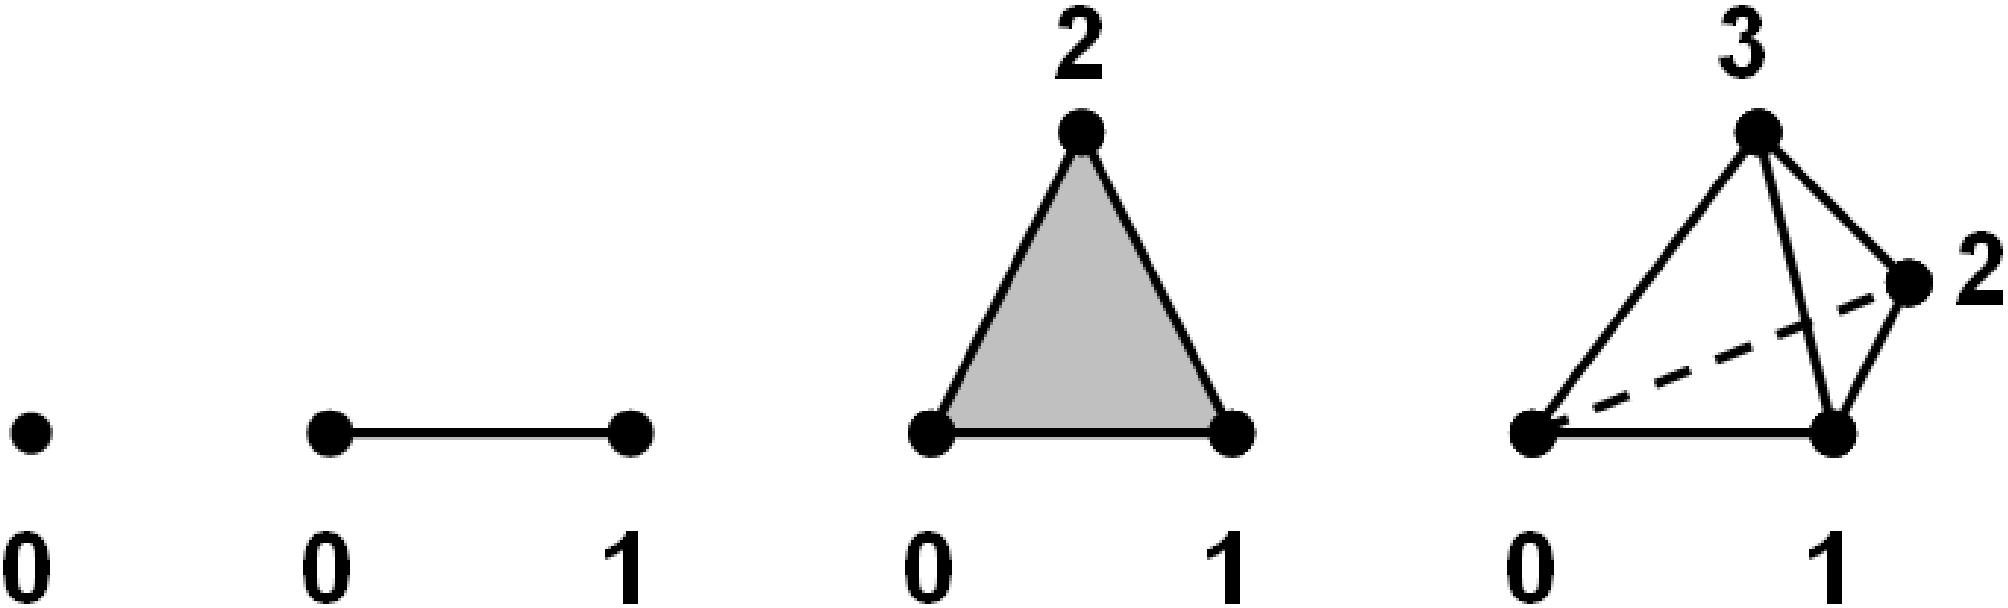
\includegraphics[width=0.7\textwidth]{figures/simp2.jpg} \caption{Examples of
  $n$-simplices for $0\leq n\leq 3$.
  Image taken from~\cite{Friedman08}.}
\label{fig_simplices} \end{figure}

In topology, we often consider spaces up to \emph{homeomorphism}.
Let $X$ and
$Y$ be topological spaces.
A map $f: X\to Y$ is a \emph{homeomorphism} if it is
a continuous bijection with a continuous inverse.
For example, there is
a homeomorphism between a circle and an ellipse, but not between a circle and an
interval.
Note that homeomorphisms consider only the open sets of the space,
and are not affected by any metric or other structure on the space.
Geometric
$n$-simplices have the property that for any two simplices $T$ and $U$, $T$ and
$U$ are homeomorphic.

We can describe manifolds as simplicial complexes by decomposing them into
simplices.
A \emph{geometric simplicial complex} $X$ is a collection of
simplices in $\RR^N$ such that (a) for any simplex in $X$, all of its faces are
also in $X$, and (b) for any two simplices in $X$, their intersection is either
empty or is a face of both of them.
Note that, up to homeomorphism, we can
describe $X$ by listing the vertices of each simplex.
Common vertices then
allow us to recover which simplices share faces.

Generalising this idea, as simplices are defined by their vertices, an
(abstract) \emph{simplicial complex} $X$ is a series of sets $X^i$ ($i\geq 0$)
such that the elements of $X^n$ (the $n$-simplices) are $(n+1)$-element sets
that satisfy the following condition: for any $\{x_i\}_{i=0}^n\in X^n$, any
$n$-element subset of this set is in $X^{n-1}$.
Note that different simplices
can have common elements, which indicates they have vertices, edges, or other
sub-faces in common.
For example, we can describe a square $S$, formed by
gluing two triangles together, by \begin{align*} S^0	&=
  \{\{a\},\{b\},\{c\},\{d\}\} & S^1	&= \{\{a, b\}, \{a, c\}, \{a, d\}, \{b, c\},
  \{c, d\}\}\\ S^2	&= \{\{a,b,c\}, \{a,c,d\}\}.
\end{align*} We can describe the
simplicial complex $X$ depicted in Figure~\ref{fig_simplicial_complex} by
\begin{align*} X^0	&= \{\{v_0\}, \{v_1\}, \{v_2\}, \{v_3\}, \{v_4\},
  \{v_5\}\}\\ X^1	&= \{\{v_0, v_1\}, \{v_0, v_2\}, \{v_0, v_5\}, \{v_1, v_2\},
  \{v_2, v_3\}, \{v_2, v_4\}, \{v_2, v_5\}, \{v_3, v_4\}\}\\ X^2	&= \{\{v_0,
  v_1, v_2\}, \{v_0, v_2, v_5\}, \{v_2, v_3, v_4\}\}.
\end{align*}

\begin{figure} \centering
  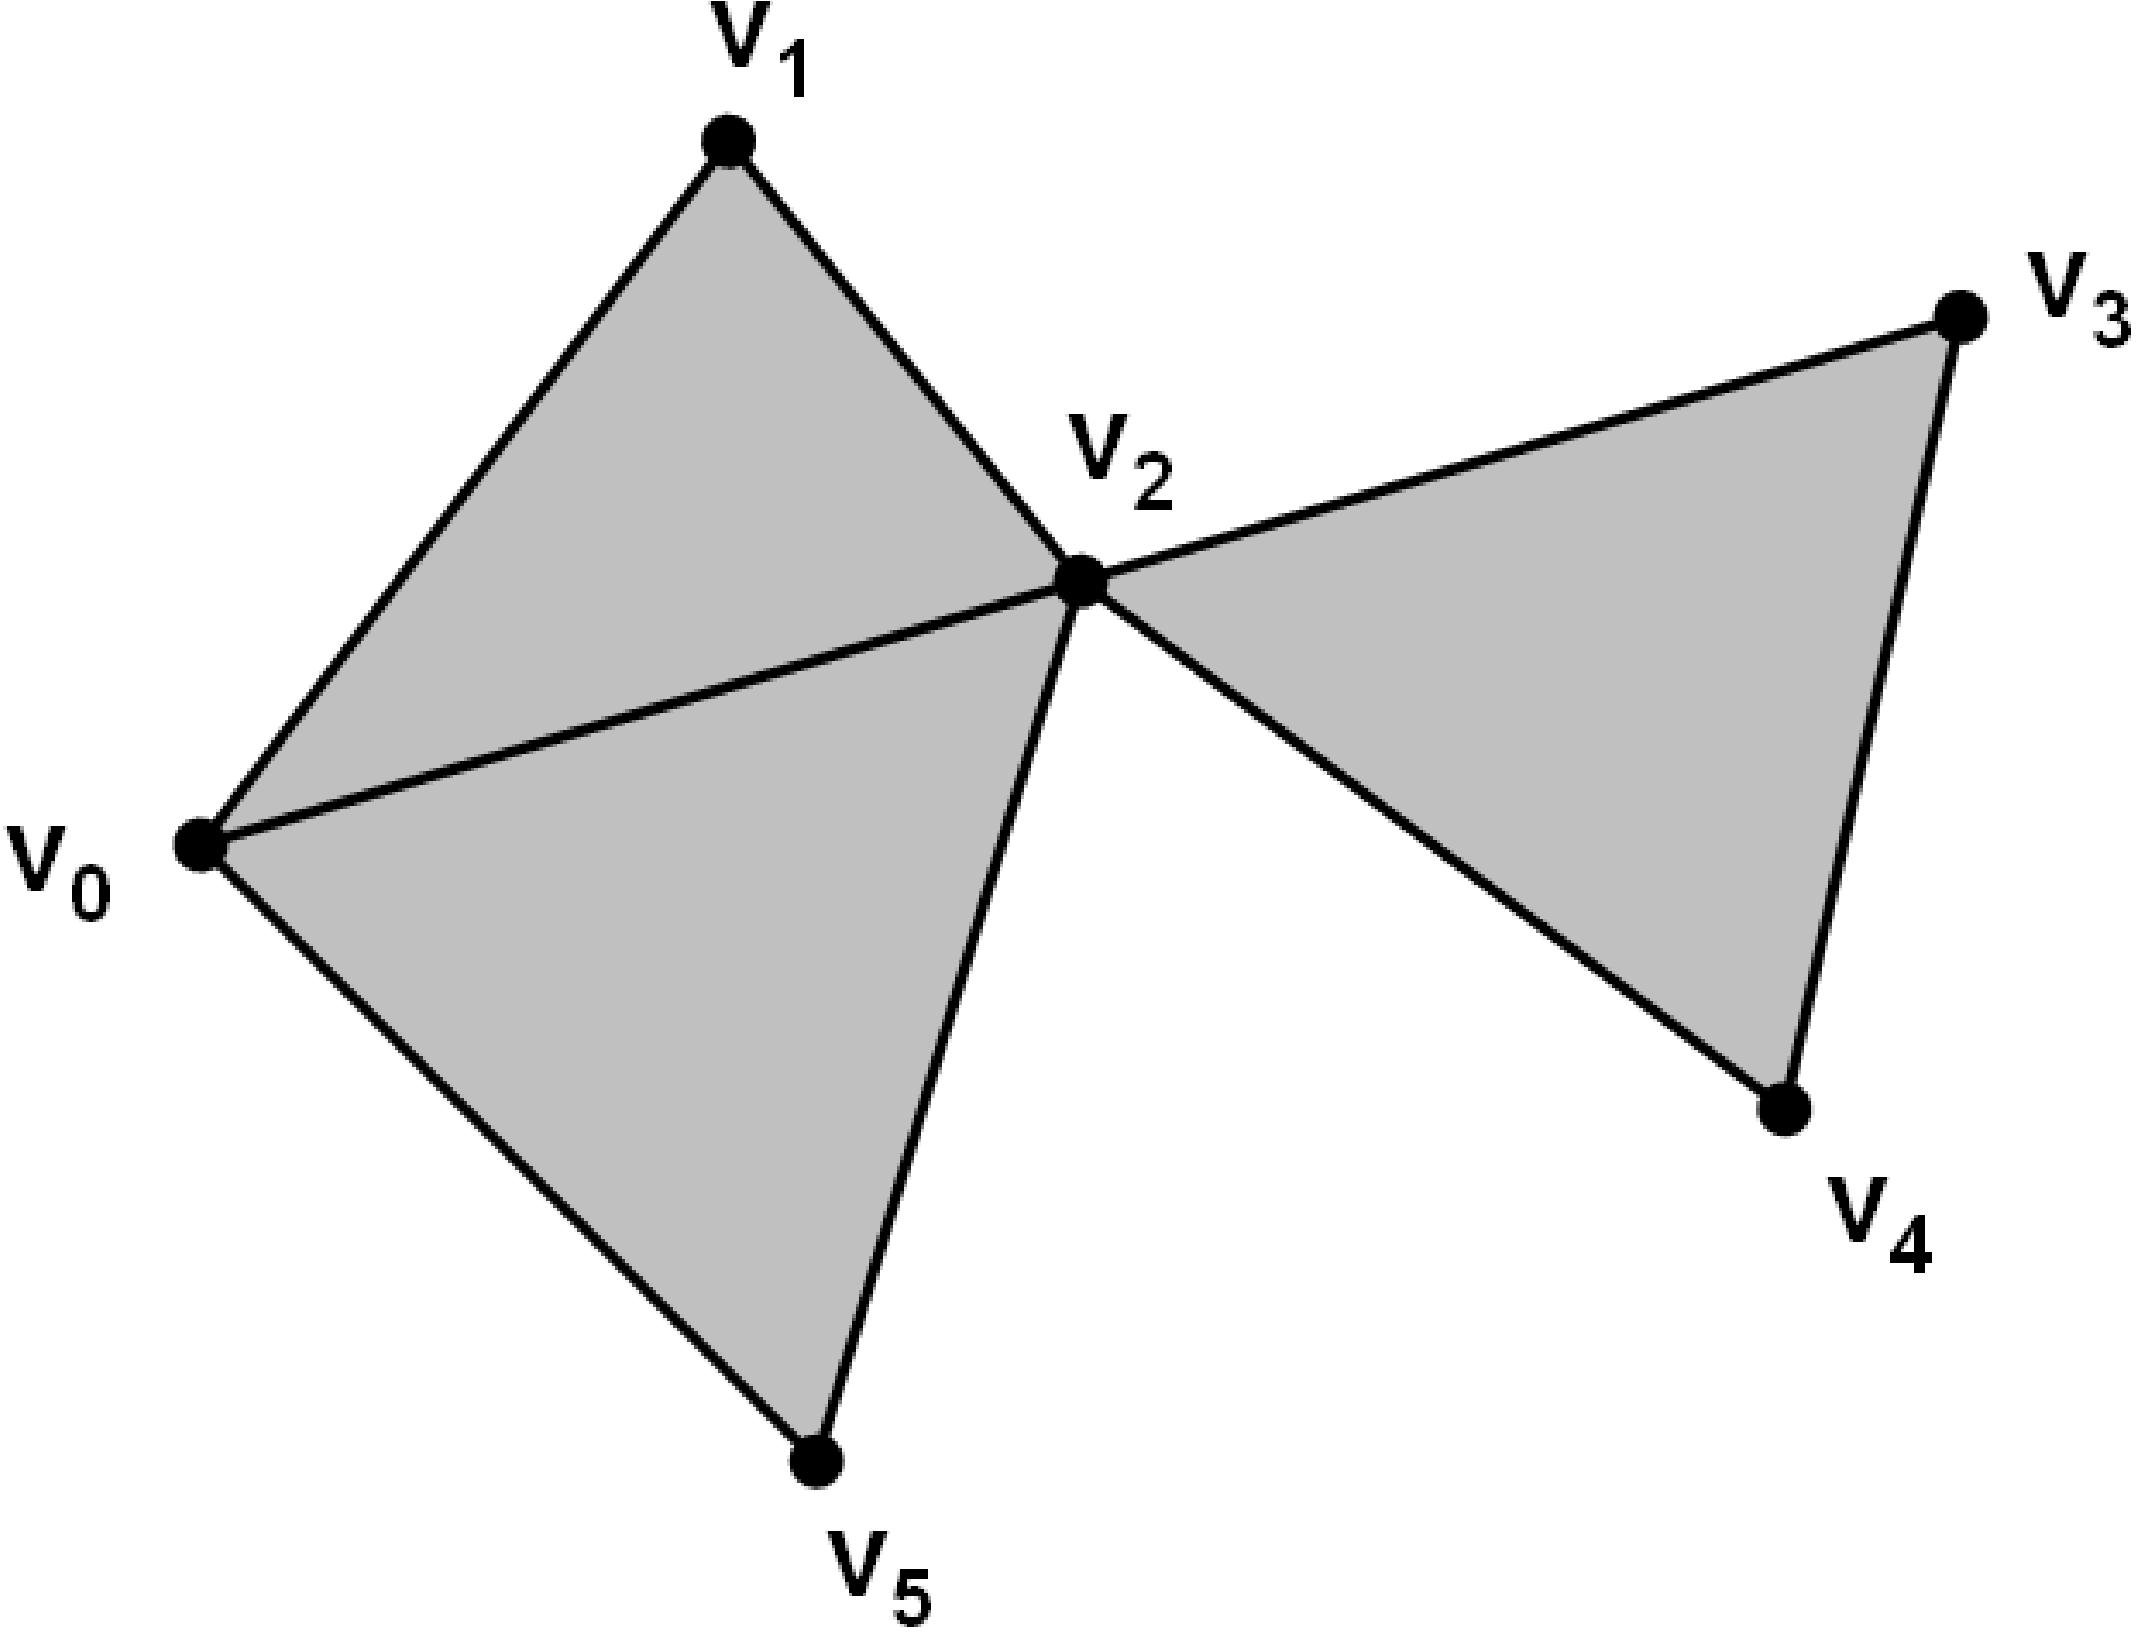
\includegraphics[width=0.4\textwidth]{figures/simp1.jpg} \caption{A simplicial
  complex $X$.
  Image taken from~\cite{Friedman08}.} \label{fig_simplicial_complex}
\end{figure}

To abstract this idea further, let all abstract simplices come with an ordering
on its vertices.
Write an (ordered) $n$-simplex as $[x_0,\dots,x_n]$.
Note
that we can characterise an $n$-simplex in a simplicial complex by its $n+1$
\emph{face maps}, where the $i^{th}$ face map sends the simplex to the face
$[x_0,\dots, x_{i-1},x_{i+1},\dots, x_n]$; that is, it sends the simplex to the
face formed by removing the $i^{th}$ vertex from the original simplex.
Let
$d_i$ be the $i^{th}$ face map.\footnote{ Note that $d_i$ is not a map of
topological spaces.
It is a formal map that to a simplex assigns its $i^{th}$
face.
Properly, we should write $d_i^n$ for the $i^{th}$ face map on
$n$-simplices.
We omit the $n$ as it is almost always clear from the context.
} One can check that we have the relation that, for $i \leq j$, $d_id_j
= d_{j-1}d_i$.
Now we can give the following definition: a \emph{Delta complex}
$X$ is a collection of sets $X^i$ with, for each $n\geq 0$ and $0\leq i\leq n$,
a map $d_i: X^{n}\to X^{n-1}$ satisfying the relation $d_id_j = d_{j-1}d_i$ for
all $i\leq j$.

We interpret the elements of $X^n$ as the $n$-simplices of the Delta complex.
The difference between Delta complexes and simplicial complexes is that in
simplicial complexes, simplices are identified by their vertex set, while in
Delta complexes, two distinct simplices may share the same vertex set.
%For example, the cone depicted in Figure~\ref{fig_cone} is a Delta complex but
%not a simplicial complex.

We can define Delta complexes in category theoretic language.
Let
$\hat{\Delta}$ be the category whose elements are the finite ordered sets $[n]
= [0,1,\ldots, n]$ and morphisms are strictly order-preserving maps $[m]\to
[n]$.
Then a Delta complex is a functor $X: \hat{\Delta}^{op}\to \textbf{Set}$.

We can translate between our two definitions of Delta complex as follows.
The
set $X([n])$ is the $n$-simplices of the Delta complex.
A map in
$\hat{\Delta}^{op}$ from $[n]$ to $[n-1]$, which is the opposite of an
order-preserving injection, is then a face map.
We can write maps from $[m]\to
[n]$ in $\hat{\Delta}$ as compositions of maps $[k]\to [k+1]$, so in general the
images of the morphisms under $X$ are compositions of face maps.

Now we will define a simplicial set.
Let $\Delta$ be the category whose
elements are the finite ordered sets $[n]$, and whose morphisms are
order-preserving maps $[m]\to [n]$.
(Compare to $\hat{\Delta}$ where the
morphisms are strictly order-preserving maps.) A \emph{simplicial set} is
a functor $X: \Delta^{op}\to \textbf{Set}$.

The difference between a Delta complexes and a simplicial set is that in
a simplicial set, we allow degenerate simplices.
For example, in $\Delta$,
there is a map $[0, 1, 2]\to [0, 1]$ that takes $0\mapsto 0$, $1\mapsto 1$ and
$2\mapsto 1$.
The image of this map under a simplicial set $X$ is a map $s:
X^1\to X^2$ that takes 1-simplex (an edge) $e\in X^1$ to some ``2-simplex'' in
$X^2$.
We can interpret this 2-simplex as a \emph{degenerate} 2-simplex (a
triangle) that has been collapsed into an edge.
A simplicial set carries the
information of all its degenerate simplices.

A \emph{fuzzy set} is a generalisation of a set where, rather than elements
being either in the set or not, there is a continuous membership function which
one can think of as a probability.
It is a set of objects $A$ and a function
$\mu: A\to [0, 1]$, where if $\mu(a) = 1$, $a$ is definitely in the fuzzy set.
The category $\textbf{Fuzz}$ of fuzzy sets has fuzzy sets as objects, and maps
of sets $f: A\to B$ such that $f\of \mu(a) \geq \mu(a)$ as morphisms.\footnote{
  We can also define fuzzy sets categorically.
Let $I$ be the interval $[0, 1]$
  with the topology whose open sets are generated by intervals $[0, a)$.
Let
  $\curI$ be the category of open subsets of $I$ where the morphisms are
  inclusion maps.
Then a fuzzy set $S$ is a functor $S: \curI^{op}\to
  \textbf{Set}$ satisfying the following conditions.
We interpret $S([0, a))$ to
  be the set of elements of $S$ of membership strength at least $a$.
Let
  $\rho_{b, a}$ be the inclusion map $[0, a)\to [0, b)$ for $b\geq a$.
Then $S$
  is a fuzzy set if (a) it is a sheaf and (b) the restriction maps $S(\rho_{b,
  a})$ are injections.
See~\cite{Weng} for the definition of a sheaf in the
  category theoretic language we want here, where you replace the category of
  R-modules with with $\textbf{Set}$.} (That is, the maps are functions that
take elements of $A$ to elements of $B$ of the same or higher membership
strength.) Then a \emph{fuzzy simplicial set} is a functor $X: \Delta^{op}\to
\textbf{Fuzz}$.\footnote{ One nice property of these fuzzy simplicial sets is
that the membership strength of the face of a simplex is at least the membership
strength of the simplex.}

\section{Converting between metric spaces and fuzzy simplicial sets}
\label{section_adjunction}

We will now give the adjunction from extended pseudo-metric spaces to fuzzy
simplicial sets.

Let $x_i$ be a fixed datapoint in the dataset $D$.
Recall that, from Section~\ref{section_uniform}, using the manifold metric
based at $x_i$, we can approximate the distance based at $x_i$ between points
$x_j, x_k\in D$
by 
$$d_{x_i}(x_j, x_k) = \begin{cases}
  \frac{1}{r_i}(d_{\RR^N}(x_j, x_k)-\rho_i) & \text{if $j = i$ or $k = i$}\\
\infty	& \text{otherwise.} \end{cases}$$ 
This distance definition gives us an extended pseudo-metric space.

Let $\textbf{EPMet}$ be the category of extended pseudo-metric spaces where the
morphisms are non-expansive maps.
Let $\textbf{FinEPMet}$ be the sub-category of $\textbf{EPMet}$ whose objects
are finite extended pseudo-metric spaces.
Note that each of the pairs $(D, d_{x_i})$ for $x_i\in D$ gives an object of
$\textbf{FinEPMet}$.

Let $\textbf{sFuzz}$ be the category of fuzzy simplicial sets (which are
functors $\Delta^{op}\to \textbf{Fuzz}$) whose morphisms are natural
transformations between the functors.
Let $\textbf{Fin-sFuzz}$ be the
sub-category of $\textbf{sFuzz}$ consisting of the fuzzy simplicial sets with
a finite number of non-degenerate simplices, defined as follows.
Let $X$ be
a fuzzy simplicial set.
An element of $X([n])$ is \emph{degenerate} if its
geometric realisation is an $(n-1)$-simplex.
The number of non-degenerate
$n$-simplices of $X$ is the number of non-degenerate elements of $X([n])$ with
positive membership strength.
Thus $X$ is in $\textbf{Fin-sFuzz}$ if it has
a finite number of non-degenerate $n$-simplices.

The main theorem of~\cite{McInnes18}, which is a slight modification of the main
theorem of~\cite{Spivak}, gives a translation between these two categories.
\begin{thm} There is an adjunction between $\textbf{FinEPMet}$ and
  $\textbf{Fin-sFuzz}$ given by $FinSing: \textbf{FinEPMet}\to
  \textbf{Fin-sFuzz}$ and $FinReal: \textbf{Fin-sFuzz}\to \textbf{FinEPMet}$,
  with $FinReal\dashv FinSing$.
\end{thm} The functors in this theorem are the
  following.\footnote{ See~\cite{McInnes18} for a categorical definition of
  these functors that makes it easier to prove they are adjoint.} The functor
  $FinReal: \textbf{Fin-sFuzz}\to\textbf{FinEPMet}$ takes a finite simplicial
  set $X$ to the finite metric space $T$ whose elements are the vertices of $X$.
  The metric on $T$ is defined as follows.
Let $\mu$ be the membership strength
  function for the simplices of $X$.\footnote{ We do not define this precisely.
  See the remark after Definition 1.1 of~\cite{Spivak} for a rigorous
  definition; Spivak's characteristic form is our membership strength function.}
  For $x, y\in T$, let $A$ be the set of all subsets of $T$ containing both $x$
  and $y$.
Then $d_T(x, y) = \min_{U\in A} -\log(\mu(U))$.

The functor $FinSing: \textbf{FinEPMet}\to \textbf{Fin-sFuzz}$ takes an finite
extended pseudo-metric space $Y$ to a finite fuzzy simplicial set, which is
a functor from $\Delta^{op}\to \textbf{Fuzz}$.
It acts as follows:
$FinSing(Y)([n])$ is the fuzzy set of $(n+1)$-vertex subsets of the datapoints
$\{x_{k_0},\ldots,x_{k_n}\}$ where the subset has membership strength
$$\mu(\{x_{k_0},\ldots,x_{k_n}\} = \min_{i, j} e^{-d(x_{k_i}, x_{k_j})}.$$

Given this translation, we can convert a set of datapoints $D$ to a family of
elements of $\textbf{FinEPMet}$, and from that to a family of finite fuzzy
simplicial sets $FinSing(D, d_{x_i})$ for $x_i\in D$.
Now, set the \emph{fuzzy
topological representation} of $D$ to be $$\bigcup_{i=1}^n FinSing(D, d_{x_i})$$
where the union is some choice of a union of fuzzy sets.
We know that each of
the $FinSing(D, d_{x_i})$ has the same set of objects, which are all simplices
whose vertices are in $D$.
Now, if $(A, \mu)$ and $(A, \nu)$ are two fuzzy sets
with the same underlying set of objects, one reasonable definition of the union
$(A, \mu) \cup (A, \nu)$ is $(A, (\mu\cup\nu))$ where $(\mu\cup\nu)(a) = \mu(a)
\bot \nu(a)$ for $\bot$ some t-conorm.
The current implementation of UMAP uses
$x\bot y = x+y-xy$, which is the obvious t-conorm to use if you interpret
$\mu(a)$ and $\nu(a)$ as probabilities of the simplex $a$ existing, assume these
are independent between the different local metric spaces, and do not care about
higher-dimensional simplices (as, for reasons of computational complexity, we
will not).

\section{Finding a good low-dimensional representation}

We now have a method for constructing a fuzzy simplicial set from a given set of
points in $\RR^n$.
Let the dataset $D$ be in $\RR^N$.
Let $E$ be
a low-dimensional representation of our dataset $D$ in $\RR^m$, for $m < N$.
To
evaluate how good $E$ is as a representation of $D$, we compare the fuzzy
simplicial set $X$ constructed from $D$ to one constructed from $E$.
In
constructing a fuzzy simplicial set $Y$ from $E$, note that we already know the
metric of the underlying manifold as it is $\RR^m$ itself.
Thus, $Y
= FinSing((E, d))$ where $d$ is the Euclidean metric on $\RR^m$.


Consider the sets of edges in $X$ and $Y$ as fuzzy sets.
Note that they have
the same underlying set of elements, which is all edges whose vertices are
labelled by elements of $D$, and differ only in the membership strength of the
simplices.
We define the cross-entropy $C$ of two fuzzy sets with the same
underlying elements set, $(A, \mu)$ and $(A, \nu)$, as follows~\cite[Definition
10]{McInnes18}: $$C((A, \mu), (A, \nu)) = \sum_{a\in
A}\left(\mu(a)\log\left(\frac{\mu(a)}{\nu(a)}\right)
+ (1-\mu(a))\log\left(\frac{1-\mu(a)}{1-\nu(a)}\right)\right).$$ Note that, in
our case, $\mu$ is fixed.
We can view this formula as follows:
$\mu(a)\log\left(\frac{\mu(a)}{\nu(a)}\right)$ provides the attractive force, as
it is minimised if short edges in $D$ correspond to short edges in $E$, since
the length of the edge is small if $\nu(a)$ is large.
Then
$(1-\mu(a))\log\left(\frac{1-\mu(a)}{1-\nu(a)}\right)$ provides the repulsive
force, as it is minimised if long edges in $D$ correspond to long edges in $E$.
We can then optimise the embedding using stochastic gradient descent.
Note that
$X$ and $Y$ contain many simplices of high dimension.
For reasons of
computational cost, the current implementation of UMAP only looks at the
cross-entropy of the one-dimensional simplices in $X$ and $Y$.

\section{Further reading}

The paper presenting UMAP,~\cite{McInnes18}, gives a good explanation of the
algorithm and implementation separate from its mathematical foundations.

For a geometrically-motivated definition of simplicial sets, and the realization
and singular functors in the classical (non-fuzzy) context,
see~\cite{Friedman08}.

For an introduction to category theory aimed at non-mathematicians,
see~\cite{Spivak18}.
To better understand the material discussed here, you need
familiarity with adjunctions (Definition 3.70).

Spivak's proof of the adjunction between the realization and singular functors
in the fuzzy set context in~\cite{Spivak} is much more explicit than that in the
UMAP paper.
Both assume familiarity with adjunctions.

\begin{thebibliography}{99}

  \bibitem{Friedman08} G. Friedman (2008). \textit{An elementary illustrated
    introduction to simplicial sets}, preprint, arXiv: 0809.4221.

  \bibitem{McInnes18} L. McInnes, J. Healy and J. Melville (2018). \textit{UMAP:
    Uniform manifold approximation and projection for dimension reduction},
    preprint, arXiv:1802.03426.

  \bibitem{McInnesVideo} L. McInnes (2018). \textit{Topological Approaches for
    Unsupervised Learning}, talk at Machine Learning Prague, accessed at
    \url{https://slideslive.com/38913519/topological-approaches-for-unsupervised-learning}.

  \bibitem{McInnesBenchmarking} L. McInnes (2018). \textit{Performance
    Comparison of Dimension Reduction Implementations}, accessed at
    \url{https://umap-learn.readthedocs.io/en/latest/benchmarking.html}.

  \bibitem{McInnesGithub} L. McInnes (2019). \textit{UMAP: Uniform manifold
    approximation and projection}, accessed at
    \url{https://github.com/lmcinnes/umap}.

  \bibitem{Melville} J. Melville (2018). \textit{UMAP Examples}, accessed at
    \url{https://jlmelville.github.io/uwot/umap-examples.html}.

  \bibitem{MelvilleGithub} J. Melville (2019). \textit{UWOT: An R package
    implementing the UMAP dimensionality reduction method}, accessed at
    \url{https://github.com/jlmelville/uwot}.

  \bibitem{Riehl} E. Riehl (2014). \textit{Category Theory in Context}, accessed
    at \url{http://www.math.jhu.edu/~eriehl/context.pdf}.

  \bibitem{Spivak18} B. Fong and D. Spivak (2018). \textit{Seven Sketches in
    Compositionality: An Invitation to Applied Category Theory}, accessed at
    \url{http:// math.mit.edu/~dspivak/teaching/sp18/7Sketches.pdf}.

  \bibitem{Spivak} D. Spivak. \textit{Metric realization of fuzzy simplicial
    sets}, accessed at
    \url{http://math.mit.edu/~dspivak/files/metric_realization.pdf}.

  \bibitem{Weng} D. Weng. \textit{A categorical introduction to sheaves},
    accessed at
    \url{http://www.math.uchicago.edu/~may/VIGRE/VIGRE2011/REUPapers/WengD.pdf}.

\end{thebibliography}

\end{document}
